\documentclass[tikz]{standalone}

\usetikzlibrary{arrows.meta,positioning}

\begin{document}
	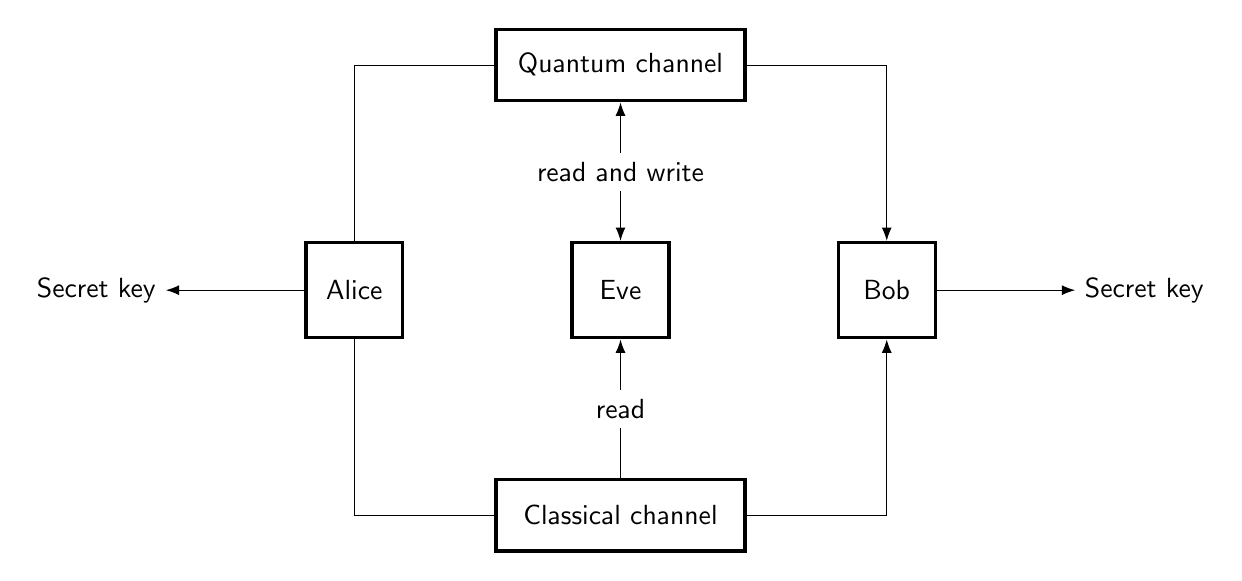
\begin{tikzpicture}[
		node distance=5em,
		party/.style={draw, very thick, fill=white, minimum height=8ex, minimum width=3.5em},
		channel/.style={party, minimum height=6ex, minimum width=9em},
	]
		\coordinate (in) at (0,0);
		\node (alice) [party, right=of in] {\textsf{Alice}};
		\node (eve) [party, right=6em of alice] {\textsf{Eve}};
		\node (bob) [party, right=6em of eve] {\textsf{Bob}};
		\coordinate[right=of bob] (out);
		
		\node (qch) [channel, above=of eve, ] {\textsf{Quantum channel}};
		\node (cch) [channel, below=of eve, minimum height=6ex, minimum width=9em] {\textsf{Classical channel}};
		
		\draw[-Latex] (alice.north) -- (alice.north|-qch) -- (qch) -- (qch-|bob.north) -- (bob.north);
		\draw[-Latex] (alice.south) -- (alice.south|-cch) -- (cch) -- (cch-|bob.south) -- (bob.south);
		
		\draw[Latex-Latex] (eve) -- (qch) node[midway, fill=white]{\textsf{read and write}};
		\draw[Latex-] (eve) -- (cch) node[midway, fill=white]{\textsf{read}};
		
		\draw[-Latex] (bob) -- (out) node[right]{\textsf{Secret key}};
		\draw[-Latex] (alice) -- (in) node[left]{\textsf{Secret key}};
	\end{tikzpicture}
\end{document}
